\subsubsection{الگوی \lr{Triple Modular Redundancy}}
\label{archSafeTripModRedunSec}
\begin{RTL}
الگوی تکرار سه‌گانه مدولار \lr{(TMR)} \cite{ref4} با استفاده از سه کانال
موازی برای پردازش تسک‌ها، مقایسه خروجی‌ها و اعمال قانون دو از سه
در صورت اختلاف، قابلیت اطمینان و ایمنی را افزایش می‌دهد. این الگو به
سیستم اجازه می‌دهد تا در حضور خطاهای تصادفی بدون از دست دادن داده‌های
ورودی یا نیاز به زمان اضافی برای تصحیح، به کار خود ادامه دهد.
در حالی که هدف آن محافظت در برابر خطاهای تصادفی مشابه
\nameref{archSafeHomoRedundancySec} است، عملیات موازی
\lr{TMR} آن را از نظر زمانی کارآمدتر می‌کند.
با این حال، بدون استفاده از کانال‌های ناهمگن، از خطاهای سیستماتیک
محافظت نمی‌کند. \lr{TMR} به دلیل تکرار سخت‌افزار هزینه بالایی دارد،
اما برای برنامه‌های بسیار حیاتی با نیاز به قابلیت اطمینان بالا
و بدون وضعیت ایمن ضروری است.
\end{RTL}
\begin{figure}[h!]
\centering
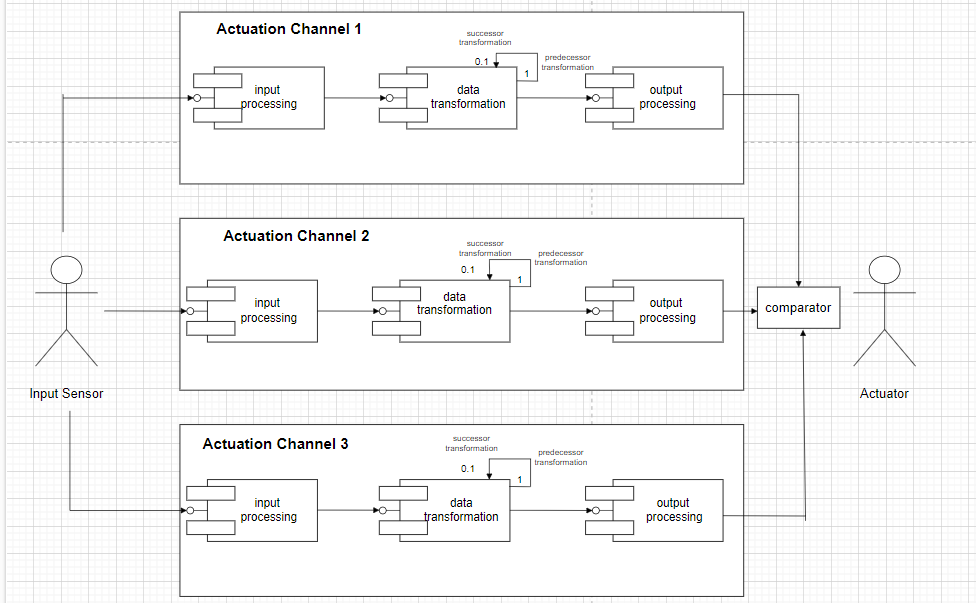
\includegraphics[scale=0.5]{images/second/triple.png}
\caption{ساختار الگوی \lr{Triple Modular Redundancy}}
\end{figure}